\documentclass[14pt]{extarticle}
\usepackage{fontspec}
\usepackage{polyglossia}
\usepackage{amsmath}
\usepackage{amssymb}
\usepackage{xcolor}
\usepackage{fancyhdr}
\usepackage{graphicx}
\usepackage{listings}
\usepackage[most]{tcolorbox}
% \usepackage{setspace}
\usepackage{pifont}
\usepackage{enumitem}
\usepackage{titlesec}
\usepackage[bottom]{footmisc}
\usepackage{titling}
\usepackage{minted}
\usepackage{etoolbox}
\usepackage{array}
\usepackage{extsizes}
\usepackage{float}
\usepackage{booktabs}
\usepackage{hyperref}
\usepackage[onehalfspacing]{setspace}
\newif\ifcolorblind
\ifdefined\setcolorblind
  \setcolorblind
\fi

\ifcolorblind
  \usepackage[a4paper, landscape, top=1cm, bottom=1cm, left=1cm, right=1cm, headheight=1.5cm, headsep=0.5cm]{geometry}
\else
  \usepackage[a4paper, top=2.7cm, bottom=2.7cm, left=2.5cm, right=2.5cm, headheight=1.5cm, headsep=0.5cm]{geometry}
\fi
\usepackage{tikz}
\usepackage{datetime2}

\usetikzlibrary{automata, positioning, arrows.meta, arrows}

\newfontfamily\emoji{Segoe UI Emoji}

\pagestyle{fancy}

\setmainlanguage[numerals=western]{arabic}
\setotherlanguage{english}
\newfontfamily\arabicfont[Script=Arabic]{Calibri}
\newfontfamily\arabicfonttt[Script=Arabic]{Courier New}



\ifcolorblind
\lstset{
  language=[Sharp]C,
  numbers=left,
  stepnumber=1,
  numbersep=8pt,
  frame=single,
  basicstyle=\ttfamily\small,
  keywordstyle=\bfseries,
  stringstyle=\ttfamily,
  commentstyle=\itshape
}
\else
\lstset{
  language=[Sharp]C,
  numbers=left,
  stepnumber=1,
  numbersep=8pt,
  frame=single,
  basicstyle=\ttfamily\small,
  keywordstyle=\color{blue},
  stringstyle=\color{red},
  commentstyle=\color{green!50!black}
}
\fi

\newif\ifdetailed
\ifdefined\setdetailed
  \setdetailed
\fi

\newif\ifwithsols
\ifdefined\setwithsols
  \setwithsols
\fi

\ifcolorblind
  \AtBeginDocument{
    \LARGE
    \usemintedstyle{bw}
  }
\fi

% unified tcolorboxes for articles
\ifcolorblind
\tcbset{colback=white, colframe=black, fonttitle=\bfseries, boxrule=1pt}
\newtcolorbox{boxDef}[1][]{title={{\emoji📘} تعريف\ifx\\#1\\\else ~#1\fi :}}
\newtcolorbox{boxExercise}[1][]{title={{\emoji🧩} تمرين\ifx\\#1\\\else ~#1\fi :}}
\newtcolorbox{boxExample}[1][]{title={{\emoji📝} مثال\ifx\\#1\\\else ~#1\fi :}}
\newtcolorbox{boxNote}[1][]{title={{\emoji✨} ملاحظة\ifx\\#1\\\else ~#1\fi :}}
\newtcolorbox{boxAttention}[1][]{title={{\emoji🔔} تنبيه\ifx\\#1\\\else ~#1\fi :}}
\newtcolorbox{boxWarning}[1][]{title={{\emoji⚡} ملاحظة هامة\ifx\\#1\\\else ~#1\fi :}}
\newtcolorbox{boxSolution}[1][]{title={{\emoji✅} حل\ifx\\#1\\\else ~#1\fi :}}
\newtcolorbox{boxSymbol}[1][]{title={{\emoji🔣} رمز\ifx\\#1\\\else ~#1\fi :}}
\newtcolorbox{boxHint}[1][]{title={{\emoji💡} تلميح\ifx\\#1\\\else ~#1\fi :}}
\else
\tcbset{colback=white, colframe=black, fonttitle=\bfseries, boxrule=0.8pt}
\newtcolorbox{boxDef}[1][]{colback=blue!5!white,colframe=blue!75!black,
  title={{\emoji📘} تعريف\ifx\\#1\\\else ~#1\fi :}}
\newtcolorbox{boxExercise}[1][]{colback=cyan!5!white,colframe=cyan!70!black,
  title={{\emoji🧩} تمرين\ifx\\#1\\\else ~#1\fi :}}
\newtcolorbox{boxExample}[1][]{colback=yellow!5!white,colframe=orange!90!black,
  title={{\emoji📝} مثال\ifx\\#1\\\else ~#1\fi :}}
\newtcolorbox{boxNote}[1][]{colback=gray!10!white,colframe=black,
  title={{\emoji✨} ملاحظة\ifx\\#1\\\else ~#1\fi :}}
\newtcolorbox{boxAttention}[1][]{colback=magenta!10!white,colframe=magenta!80!black,
  title={{\emoji🔔} تنبيه\ifx\\#1\\\else ~#1\fi :}}
\newtcolorbox{boxWarning}[1][]{colback=red!5!white,colframe=red!75!black,
  title={{\emoji⚡} ملاحظة هامة\ifx\\#1\\\else ~#1\fi :}}
\newtcolorbox{boxSolution}[1][]{colback=green!5!white,colframe=green!60!black,
  title={{\emoji✅} حل\ifx\\#1\\\else ~#1\fi :}}
\newtcolorbox{boxSymbol}[1][]{colback=purple!5!white,colframe=purple!70!black,
  title={{\emoji🔣} رمز\ifx\\#1\\\else ~#1\fi :}}
\newtcolorbox{boxHint}[1][]{colback=teal!5!white,colframe=teal!60!black,
  title={{\emoji💡} تلميح\ifx\\#1\\\else ~#1\fi :}}
\fi


\ifcolorblind
\tcbset{simplecode/.style={ colback=white, colframe=black, boxrule=1pt, arc=2pt, left=4pt,right=4pt,top=4pt,bottom=4pt}}
\else
\tcbset{simplecode/.style={ colback=gray!5, colframe=black!50, boxrule=0.4pt, arc=2pt, left=4pt,right=4pt,top=4pt,bottom=4pt}}
\fi
\newenvironment{boxCode}{\begin{tcolorbox}[simplecode]}{\end{tcolorbox}}

\newcolumntype{C}[1]{>{\centering\arraybackslash}p{#1}}

\makeatletter
\DTMnewdatestyle{dotted}{%
  \renewcommand{\DTMdisplaydate}[4]{\two@digits{##3}.\two@digits{##2}.##1}%
  \renewcommand{\DTMDisplaydate}{\DTMdisplaydate}%
}
\makeatother
\DTMsetdatestyle{dotted}

% redefine spaces after titles
\makeatletter
\renewcommand{\@maketitle}{%
  \begin{center}
    {\huge \bfseries \@title \par}%
    \vskip 0.2em % space between title and author
    {\large \@author \par}%
    % \vskip 0.2em % space between author and date
    % {\normalsize \@date \par}%
    {\small \hfill \begin{english}\DTMtoday\end{english} \par}%
  \end{center}
}
\makeatother

\fancyhf{} % clear default
\fancypagestyle{plain}{
  \fancyhf{}
  \fancyhead[L]{مدرسة التسامح الشاملة}
  % \fancyhead[L]{
\includegraphics[height=1cm]{../../../images/logoTasamoh.png}}
  \fancyhead[R]{الأستاذ محمود اغبارية}
  \fancyfoot[C]{\thepage}
}

\fancyhead[L]{مدرسة التسامح الشاملة}
\fancyhead[R]{الأستاذ محمود اغبارية}
\fancyfoot[C]{\thepage}

\setcounter{tocdepth}{3} % only section subsection and subsubsection in TOC

\newcommand{\importpdfpage}[2]{%
    \thispagestyle{empty}
    \newgeometry{left=0cm,right=0cm,top=0cm,bottom=0cm}
    \includegraphics[page=#2,width=0.95\paperwidth,height=0.95\paperheight,keepaspectratio]{#1}
    \restoregeometry
}

\newcommand{\insertFullImg}[1]{%
    \noindent
    \makebox[\textwidth][c]{
        \includegraphics[width=0.9\paperwidth,keepaspectratio]{#1}%
    }%
}%

% ----------------------


% \begin{document}

% \maketitle

% % \clearpage  % start TOC on a new page
% % \renewcommand{\contentsname}{جدول المحتويات}
% % \tableofcontents
% % \clearpage

% \part*{part 1} % the * prevents numbering
% \section*{مقدمة}
% \subsection*{مثال رياضي}
% \subsubsection*{مثال فرعي}
% \paragraph*{ paragraph 1}
% \subparagraph*{sub paragraph 1}

% \ifdetailed
% \begin{english}
% \begin{minted}{csharp}
% // C# Example
% \end{minted}
% \end{english}
% \fi

% OLD WAY
% \ifdetailed
% \begin{english}
% \begin{lstlisting}
% // C# Example
% \end{lstlisting}
% \end{english}
% \fi

% % 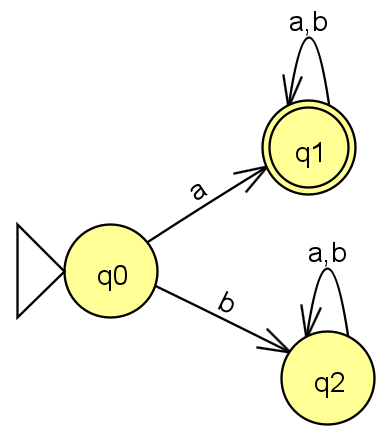
\includegraphics[width=0.2\textwidth]{../../../images/DFAs/ex1_q1.png}



% \vspace{3cm}
% \begin{flushleft}
% أرجو لكم وقتًا ممتعًا.

% الأستاذ محمود اغبارية.
% \end{flushleft}


% \end{document}


\ifwithsols
\title{حل ورقة عمل مراجعة شاملة - مادة بايثون (أ)}
\else
\title{ورقة عمل مراجعة شاملة - مادة بايثون (أ)}
\fi

\begin{document}

\maketitle
\thispagestyle{fancy}

\section*{الموضوع 1: العمليات، المتغيرات، والمدخلات/المخرجات (\textenglish{def, input, print})}
\begin{enumerate}[itemsep=3em]

\item
أمامك كود يستقبل معلومات عن مدرسة:
\begin{boxCode}
\begin{english}
\begin{minted}{python}
def school_info():
    school_name = input('Enter school name: ')
    students_count = int(input('Enter students count: '))
    print('School:', school_name, 'Students:', students_count + 10)

school_info()
\end{minted}
\end{english}
\end{boxCode}
\begin{enumerate}
    \item ما هو المخرج المطبوع على الشاشة بالتفصيل إذا أدخل المستخدم اسم المدرسة '\textenglish{Ibn Haytham}' والعدد '\textenglish{300}'؟
    \item ما هي وظيفة الأمر \textenglish{int()} في السطر الثاني؟
\end{enumerate}

\ifwithsols
\begin{boxSolution}
\begin{enumerate}
    \item \textenglish{School: Ibn Haytham Students: 310}
    \item يقوم بتحويل القيمة المدخلة (نص) إلى عدد صحيح.
\end{enumerate}
\end{boxSolution}
\fi

\item
أمامك الكود التالي:
\begin{boxCode}
\begin{english}
\begin{minted}{python}
def greet():
    name = input()
    age = int(input())
    print(name, age + 2)

greet()
\end{minted}
\end{english}
\end{boxCode}
\begin{enumerate}
    \item ما المخرج المطبوع إذا أدخل المستخدم الاسم 'أحمد' والعمر '\textenglish{14}'؟
    \item ما أهمية استخدام الأمر \textenglish{int()} في السطر الثالث؟
\end{enumerate}

\ifwithsols
\begin{boxSolution}
\begin{enumerate}
    \item أحمد \textenglish{16}
    \item يقوم بتحويل القيمة المدخلة (نص) إلى عدد صحيح.
\end{enumerate}
\end{boxSolution}
\fi

\item
اكتب دالة باسم \textenglish{rectangle(a, b)} تستقبل طولي ضلعين لمستطيل (أعداد صحيحة)، وتقوم بحساب مساحة المستطيل ومحيطه وطباعتهما في رسالة توضيحية للمستخدم.

\ifwithsols
\begin{boxSolution}
\begin{english}
\begin{minted}{python}
def rectangle(a, b):
    area = a * b
    perimeter = 2 * (a + b)
    print("Area:", area, "Perimeter:", perimeter)
\end{minted}
\end{english}
\end{boxSolution}
\fi

\end{enumerate}
% \clearpage

\section*{الموضوع 2: العوامل الحسابية الأساسية (+, -, *, /)}
\begin{enumerate}[itemsep=3em]

\item
احسب ناتج التعبيرات البرمجية التالية كما تتوقعها بايثون:
\begin{enumerate}[label=\arabic*)]
    \item \textenglish{print(10 + 5 * 2)}
    \item \textenglish{print((10 + 5) * 2)}
    \item \textenglish{print(20 / 4)}
\end{enumerate}
ما هو نوع البيانات الناتج في المسألة رقم (3)؟ (\textenglish{int} أم \textenglish{float}؟)

\ifwithsols
\begin{boxSolution}
\begin{enumerate}[label=\arabic*)]
    \item \textenglish{20}
    \item \textenglish{30}
    \item \textenglish{5.0}
\end{enumerate}
النوع هو \textenglish{float}.
\end{boxSolution}
\fi

\item
تتبع الحسابات التالية واذكر الناتج ونوع البيانات لـ \textenglish{a} و \textenglish{b}:
\begin{boxCode}
\begin{english}
\begin{minted}{python}
a = 20 / 4
b = a + 5 * 2
print('a =', a, 'b =', b)
\end{minted}
\end{english}
\end{boxCode}

\ifwithsols
\begin{boxSolution}
\begin{english}
a = 5.0 (float) \\
b = 15.0 (float) \\
a = 5.0 b = 15.0
\end{english}
\end{boxSolution}
\fi

\item
تتبع الكود التالي وأكمل جدول المتابعة لقيم المتغيرات \textenglish{a, b, temp}:
\begin{boxCode}
\begin{english}
\begin{minted}{python}
a = 15
b = 40
temp = a
a = b
b = temp
print('a=', a, 'b=', b)
\end{minted}
\end{english}
\end{boxCode}
\begin{enumerate}
    \item ما هي القيم النهائية المطبوعة لـ \textenglish{a} و \textenglish{b}؟
    \item اشرح بكلماتك أهمية المتغير \textenglish{temp}.
\end{enumerate}

\ifwithsols
\begin{boxSolution}
\begin{enumerate}
    \item \textenglish{a = 40, b = 15}
    \item المتغير \textenglish{temp} يستخدم كمتغير وسيط لحفظ قيمة \textenglish{a} قبل تغييرها، لكي نتمكن من إعطائها لـ \textenglish{b} لاحقاً، وبذلك تكتمل عملية التبديل (\textenglish{swap}).
\end{enumerate}
\end{boxSolution}
\fi

\item
تتبع الكود التالي وأوجد قيم المتغيرات النهائية:
\begin{boxCode}
\begin{english}
\begin{minted}{python}
x = 5
y = 10
temp = x
x = y
y = temp
print('x =', x, 'y =', y)
\end{minted}
\end{english}
\end{boxCode}
\begin{enumerate}
    \item ما القيم المطبوعة لـ \textenglish{x} و \textenglish{y}؟
    \item ما الغرض من استخدام المتغير الوسيط \textenglish{temp}؟
\end{enumerate}

\ifwithsols
\begin{boxSolution}
\begin{enumerate}
    \item \textenglish{x = 10, y = 5}
    \item التبديل بين قيمتين.
\end{enumerate}
\end{boxSolution}
\fi

\end{enumerate}
\clearpage

\section*{الموضوع 3: القسمة الصحيحة (//) وباقي القسمة (\%)}
\begin{enumerate}[itemsep=3em]

\item
جد نواتج العمليات التالية:
\begin{enumerate}[label=\arabic*)]
    \item \textenglish{print(28 // 6)}
    \item \textenglish{print(28 \% 6)}
    \item \textenglish{print(15 \% 2)}
    \item \textenglish{print(1024 // 100)}
    \item \textenglish{print(1024 \% 100)}
\end{enumerate}

\ifwithsols
\begin{boxSolution}
\begin{enumerate}[label=\arabic*)]
    \item 4
    \item 4
    \item 1
    \item 10
    \item 24
\end{enumerate}
\end{boxSolution}
\fi

\item
أراد معلم توزيع 33 هدية بالتساوي على 5 طلاب متميزين.
اكتب مقطع كود يحسب ويطبع:
\begin{enumerate}[label=\arabic*)]
    \item عدد الهدايا التي سيحصل عليها كل طالب.
    \item عدد الهدايا المتبقية لدى المعلم.
\end{enumerate}

\ifwithsols
\begin{boxSolution}
\begin{english}
\begin{minted}{python}
total_gifts = 33
students = 5
gifts_per_student = total_gifts // students
remaining_gifts = total_gifts % students

print("هدايا لكل طالب:", gifts_per_student)
print("هدايا متبقية:", remaining_gifts)
\end{minted}
\end{english}
\end{boxSolution}
\fi

\item
اكتب مقطع كود يستقبل عدداً صحيحاً من المستخدم، ويطبع الرسالة '\textenglish{Even}' إذا كان العدد زوجياً، والرسالة '\textenglish{Odd}' إذا كان فردياً.

\ifwithsols
\begin{boxSolution}
\begin{english}
\begin{minted}{python}
num = int(input("Enter a number: "))
if num % 2 == 0:
    print("Even")
else:
    print("Odd")
\end{minted}
\end{english}
\end{boxSolution}
\fi

\end{enumerate}
\clearpage

\section*{الموضوع 4: الشرط البسيط وعوامل المقارنة (\textenglish{if, else, ==, !=, <, >})}
\begin{enumerate}[itemsep=3em]

\item
حدد نتيجة كل تعبير منطقي مما يلي (\textenglish{True} أو \textenglish{False}):
\begin{enumerate}[label=\arabic*)]
    \item \textenglish{54 == 54}
    \item \textenglish{100 < 50}
    \item \textenglish{'Python' == 'python'}
    \item \textenglish{100 != 200}
    \item \textenglish{50 == 50}
    \item \textenglish{100 < 40}
    \item \textenglish{'abc' != 'ABC'}
    \item \textenglish{15 >= 15}
\end{enumerate}

\ifwithsols
\begin{boxSolution}
\begin{enumerate}[label=\arabic*)]
    \item True
    \item False
    \item False
    \item True
    \item True
    \item False
    \item True
    \item True
\end{enumerate}
\end{boxSolution}
\fi

\item
اكتب برنامجاً (\textenglish{grade}) يستقبل درجة الطالب في امتحان الحاسوب:
\begin{itemize}
    \item إذا كانت الدرجة 60 أو أكثر، يطبع الرسالة: '\textenglish{Pass} - ناجح'.
    \item خلاف ذلك، يطبع الرسالة: '\textenglish{Try again} - حاول مجدداً'.
\end{itemize}

\ifwithsols
\begin{boxSolution}
\begin{english}
\begin{minted}{python}
grade = int(input("Enter your grade: "))
if grade >= 60:
    print("Pass - ناجح")
else:
    print("Try again - حاول مجدداً")
\end{minted}
\end{english}
\end{boxSolution}
\fi

\item
اكتب برنامجاً (\textenglish{age}) يستقبل عمر شخص:
\begin{itemize}
    \item إذا كان العمر 18 أو أكثر، يطبع الرسالة: '\textenglish{Adult}'.
    \item خلاف ذلك، يطبع الرسالة: '\textenglish{Minor}'.
\end{itemize}

\ifwithsols
\begin{boxSolution}
\begin{english}
\begin{minted}{python}
age = int(input("Enter your age: "))
if age >= 18:
    print("Adult")
else:
    print("Minor")
\end{minted}
\end{english}
\end{boxSolution}
\fi

\end{enumerate}
\clearpage

\section*{الموضوع 5: الشرط المركب والعوامل المنطقية (\textenglish{and, or, not})}
\begin{enumerate}[itemsep=3em]

\item
حدد نتيجة التقييم المنطقي للتعابير التالية (\textenglish{True / False}):
\begin{enumerate}[label=\arabic*)]
    \item \textenglish{(3 < 5) and (9 > 10)}
    \item \textenglish{(8 < 7) or (16 > 15)}
    \item \textenglish{not (10 == 10)}
    \item \textenglish{(4 <= 4) and not (5 < 2)}
    \item \textenglish{(5 > 3) and (2 > 10)}
    \item \textenglish{(5 > 3) or (2 > 10)}
\end{enumerate}

\ifwithsols
\begin{boxSolution}
\begin{enumerate}[label=\arabic*)]
    \item False
    \item True
    \item False
    \item True
    \item False
    \item True
\end{enumerate}
\end{boxSolution}
\fi

\item
اكتب برنامجاً يستقبل المبلغ المالي الموفر (\textenglish{savings}) وعدد أشهر التوفير (\textenglish{months}).
يطبع البرنامج الرسالة: 'أصبح باستطاعتك شراء حاسوب محمول!' إذا كان المبلغ أكثر من 4000 ش.ج أو كان عدد الأشهر أكثر من 10 أشهر.

\ifwithsols
\begin{boxSolution}
\begin{english}
\begin{minted}{python}
savings = float(input("Enter savings: "))
months = int(input("Enter months: "))

if savings > 4000 or months > 10:
    print("أصبح باستطاعتك شراء حاسوب محمول!")
\end{minted}
\end{english}
\end{boxSolution}
\fi

\item
اكتب برنامجاً يستقبل رقماً صحيحاً من المستخدم، ويطبع '\textenglish{Valid}' إذا كان الرقم بين 10 و 50 (يشمل) وكان زوجيّاً بنفس الوقت.

\ifwithsols
\begin{boxSolution}
\begin{english}
\begin{minted}{python}
num = int(input("Enter number: "))

if num >= 10 and num <= 50 and num % 2 == 0:
    print("Valid")
\end{minted}
\end{english}
\end{boxSolution}
\fi

\end{enumerate}
\clearpage

\section*{الموضوع 6: الشرط المتداخل والشرط المتعدد (\textenglish{nested if, if-elif-else})}
\begin{enumerate}[itemsep=3em]

\item
أمامك مقطع كود لحساب سعر وجبة مطعم برجر:
\begin{boxCode}
\begin{english}
\begin{minted}{python}
meal = 'عائلية'
if meal == 'شخصية':
    price = 52
elif meal == 'عائلية':
    price = 120
else:
    price = 42
print('السعر النهائي:', price)
\end{minted}
\end{english}
\end{boxCode}
\begin{enumerate}
    \item ما هو المخرج المطبوع عند تشغيل الكود أعلاه؟
    \item ماذا سيكون المخرج إذا تم تغيير القيمة إلى \textenglish{meal = 'أطفال'}؟
\end{enumerate}

\ifwithsols
\begin{boxSolution}
\begin{enumerate}
    \item السعر النهائي: 120
    \item السعر النهائي: 42
\end{enumerate}
\end{boxSolution}
\fi

\item
اكتب برنامجاً يستقبل معدل طالب في المدرسة (\textenglish{avg}):
\begin{itemize}
    \item إذا كان المعدل 90 فما فوق، يطبع: '\textenglish{Excellent}'.
    \item إذا كان المعدل بين 75 و 89 (يشمل)، يطبع: '\textenglish{Very Good}'.
    \item إذا كان بين 60 و 74 (يشمل)، يطبع: '\textenglish{Good}'.
    \item إذا كان أقل من 60، يطبع: '\textenglish{Needs Improvement}' أو '\textenglish{Pass}'.
\end{itemize}

\ifwithsols
\begin{boxSolution}
\begin{english}
\begin{minted}{python}
avg = float(input("Enter average: "))
if avg >= 90:
    print("Excellent")
elif avg >= 75 and avg <= 89:
    print("Very Good")
elif avg >= 60 and avg <= 74:
    print("Good")
else:
    print("Needs Improvement")
\end{minted}
\end{english}
\end{boxSolution}
\fi

\end{enumerate}
\clearpage

\section*{الموضوع 7: حلقة التكرار المحددة \textenglish{for} والدالة \textenglish{range}}
\begin{enumerate}[itemsep=3em]

\item
اكتب المخرجات الدقيقة الناتجة عن المقاطع البرمجية التالية:
\begin{enumerate}
    \item
\begin{boxCode}
\begin{english}
\begin{minted}{python}
for i in range(3):
    print(i)
\end{minted}
\end{english}
\end{boxCode}
    \item
\begin{boxCode}
\begin{english}
\begin{minted}{python}
for x in range(2, 11, 3):
    print(x, end=' ')
\end{minted}
\end{english}
\end{boxCode}
    \item
\begin{boxCode}
\begin{english}
\begin{minted}{python}
for i in range(1, 10, 3):
    print(i, end=', ')
\end{minted}
\end{english}
\end{boxCode}
    \item
\begin{boxCode}
\begin{english}
\begin{minted}{python}
for x in range(3):
    print('Hello')
\end{minted}
\end{english}
\end{boxCode}
\end{enumerate}

\ifwithsols
\begin{boxSolution}
\begin{enumerate}
    \item \textenglish{0} \\ \textenglish{1} \\ \textenglish{2}
    \item \textenglish{2 5 8 }
    \item \textenglish{1, 4, 7, }
    \item \textenglish{Hello} \\ \textenglish{Hello} \\ \textenglish{Hello}
\end{enumerate}
\end{boxSolution}
\fi

\item
اكتب حلقة \textenglish{for} تقوم بحساب وطباعة مجموع الأعداد الزوجية من 2 حتى 20 (يشمل 20).

\ifwithsols
\begin{boxSolution}
\begin{english}
\begin{minted}{python}
sum_even = 0
for i in range(2, 21, 2):
    sum_even += i
print("Sum of even numbers:", sum_even)
\end{minted}
\end{english}
\end{boxSolution}
\fi

\item
اكتب حلقة \textenglish{for} تحسب وتطبع مجموع الأعداد الفردية من 1 حتى 15 (يشمل 15).

\ifwithsols
\begin{boxSolution}
\begin{english}
\begin{minted}{python}
sum_odd = 0
for i in range(1, 16, 2):
    sum_odd += i
print("Sum of odd numbers:", sum_odd)
\end{minted}
\end{english}
\end{boxSolution}
\fi

\end{enumerate}
\clearpage

\section*{الموضوع 8: حلقة التكرار المشروطة \textenglish{while} والحلقة اللانهائية}
\begin{enumerate}[itemsep=3em]

\item
حدد لكل مقطع كود مما يلي إذا كانت الحلقة منتهية (\textenglish{Finite}) أم لانهائية (\textenglish{Infinite}) مع التوضيح:
\begin{enumerate}
    \item
\begin{boxCode}
\begin{english}
\begin{minted}{python}
i = 1
while i <= 5:
    print(i)
    i += 1
\end{minted}
\end{english}
\end{boxCode}
    \item
\begin{boxCode}
\begin{english}
\begin{minted}{python}
count = 10
while count > 0:
    print(count)
\end{minted}
\end{english}
\end{boxCode}
    \item
\begin{boxCode}
\begin{english}
\begin{minted}{python}
x = 1
while x <= 5:
    print(x)
\end{minted}
\end{english}
\end{boxCode}
\end{enumerate}

\ifwithsols
\begin{boxSolution}
\begin{enumerate}
    \item حلقة منتهية. يتم زيادة قيمة \textenglish{i} بمقدار 1 في كل دورة حتى ينتفي الشرط.
    \item حلقة لانهائية. قيمة \textenglish{count} لا تتغير داخل الحلقة وتظل 10، لذا الشرط سيبقى دائمًا \textenglish{True}.
    \item حلقة لانهائية. قيمة \textenglish{x} لا تتغير داخل الحلقة وتظل 1، لذا الشرط سيبقى دائمًا \textenglish{True}.
\end{enumerate}
\end{boxSolution}
\fi

\item
اكتب برنامجاً يطلب من المستخدم إدخال أعداد صحيحة بشكل متكرر باستخدام حلقة \textenglish{while}. يتوقف البرنامج عن الاستقبال فور إدخال الرقم 0، ثم يطبع المجموع الكلي للأعداد المدخلة.

\ifwithsols
\begin{boxSolution}
\begin{english}
\begin{minted}{python}
total = 0
num = int(input("Enter a number (0 to stop): "))
while num != 0:
    total += num
    num = int(input("Enter a number (0 to stop): "))
print("Total sum:", total)
\end{minted}
\end{english}
\end{boxSolution}
\fi

\end{enumerate}
\clearpage

\section*{الموضوع 9: السلاسل النصية (\textenglish{Strings}: الفهرسة والاقتطاع)}
\begin{enumerate}[itemsep=3em]

\item
جد مخرجات الجمل البرمجية التالية إذا علمت أن \textenglish{text = 'Python'}:
\begin{enumerate}[label=\arabic*)]
    \item \textenglish{print(text[0])}
    \item \textenglish{print(text[-1])}
    \item \textenglish{print(len(text))}
    \item \textenglish{print(text[1:4])}
\end{enumerate}

\ifwithsols
\begin{boxSolution}
\begin{enumerate}[label=\arabic*)]
    \item P
    \item n
    \item 6
    \item yth
\end{enumerate}
\end{boxSolution}
\fi

\item
لتكن السلسلة النصية \textenglish{st = 'ABCDE'} (أو \textenglish{text = 'Python'}).
\begin{enumerate}
    \item اكتب أمراً برمجياً باستخدام الاقتطاع يعكس ترتيب السلسلة النصية لتصبح (\textenglish{'EDCBA'} أو \textenglish{'nohtyP'}).
    \item اكتب أمراً يطبع أول حرفين فقط.
    \item اكتب أمراً يطبع آخر حرفين فقط.
    \item اكتب أمراً يطبع النص بدون الحرف الأول والأخير.
\end{enumerate}

\ifwithsols
\begin{boxSolution}
\begin{english}
\begin{minted}{python}
# 1. Reverse the string
print(st[::-1])

# 2. First two characters
print(st[:2])

# 3. Last two characters
print(st[-2:])

# 4. Without first and last characters
print(st[1:-1])
\end{minted}
\end{english}
\end{boxSolution}
\fi

\end{enumerate}

\vspace{1cm}
\begin{flushleft}
أرجو لكم وقتًا ممتعًا.

الأستاذ محمود اغبارية.
\end{flushleft}

\end{document}
